\section{Conclusion}

    \begin{figure}[H]
        \centering
        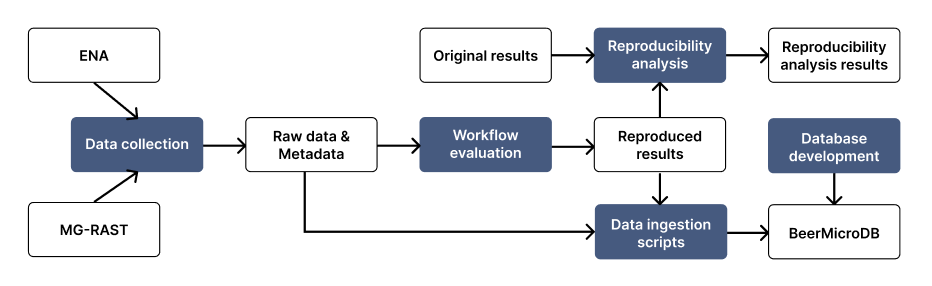
\includegraphics[scale=0.5]{images/overview.png}
        \caption{Thesis overview}
        \small In the overview of the thesis, the white box stands for the data and results, and the blue box symbolizes the action taken. The research starts with data collection, advancing to the evaluation of workflows, followed by an in-depth reproducibility analysis, and culminating in the construction of the BeerMicroDB.
        \label{fig:conclusion:overview}
    \end{figure}

    The thesis commences with the gathering of raw data and metadata from two sources: ENA and MG-RAST. Subsequently, two distinct workflows are employed: a metabarcoding workflow developed using \tool{QIIME 2} and a shotgun workflow facilitated by \tool{Kraken 2}. Both workflows have been implemented on the \tool{Galaxy} platform and automated through the Galaxy API Python library, known as \tool{BioBlend}. For the comparison of reproduced results with original findings, \tool{Jupyter Notebook} combined with \tool{Python} libraries such as \tool{Pandas}, \tool{Matplotlib}, and \tool{Seaborn} was utilized to undertake the reproducibility analysis. Based on the raw data metadata and the reproduced results, BeerMicroDB was constructed, integrating \tool{Express.js} and \tool{MongoDB} for backend operations and \tool{React.js} for frontend development.
    
    Upon the execution of the workflows, while these workflows had some variances, their overarching outcomes were in harmonious alignment with the conclusions of prior studies that we have collected. One of the principal outcomes drawn from these workflows was the evident richness in microbiome diversity observed in certain beer types, particularly those subjected to spontaneous fermentation and aging procedures. The spontaneously fermented beers include sesotho - a traditional African beer, along with Extra Doppelbock Lager and Rubi Marzen Lager. Concurrently, the aging process was predominantly linked with beers such as Blond Beer and stout beer. Contrastingly, when these beers were measured against their industrial counterparts, the distinction was clear. The aforementioned beers showcased a significantly more diverse microbiome profile. This resonates with the idea that traditional and specific brewing methods can indeed have a pronounced impact on the microbial diversity of the final product.
    
    Within the beer samples, bacterial species such as \textit{Pediococcus damnosus}, \textit{Acetobacter indonesiensis}, and \textit{Lactobacillus brevis} were predominant. On the fungal front, the dominance was held by species like \textit{Saccharomyces cerevisiae}, \textit{Wickerhamomyces anomalus}, and \textit{Pichia membranifaciens}.
    
    Our initiative to create a specialized microbiome database, named BeerMicroDB, has accumulated metadata and microbiome compositions encompassing 56 distinct beers and a total of 301 samples that are publicly available for users to browse and have an insight into beers and beer microbiomes. However, the research encountered certain limitations. The number of shotgun datasets is disproportionate relative to the metabarcoding datasets. Additionally, the \tool{QIIME 2} tool on \tool{Galaxy} currently lacks support for manifest files for data importation, given the obscured nature of data pathways in the cloud environment to its users. It's also worth noting that the present iteration of BeerMicroDB is limited to read-only access. The in-depth analysis of content in the database provided by BeerMicroDB appears to be lacking.
    
    Anticipating future advancements, there exists a keen interest in expanding the dataset spectrum, both in terms of quantity and the variety of beer types represented. Introducing more advanced statistical methods, such as principal component analysis (PCA), and potentially harnessing machine learning techniques could offer valuable insights into distinguishing the core beer microbiome associated with varying beer types or regional beer variations. Moreover, an objective lies in refining BeerMicroDB by incorporating user authentication mechanisms. This would potentially facilitate user-driven contributions, enabling them to append additional datasets and share their microbiome analysis outcomes, thereby enriching the repository.